\documentclass[spanish]{textolivre}

% metadata
\journalname{Texto Livre}
\thevolume{17}
%\thenumber{1} % old template
\theyear{2024}
\receiveddate{\DTMdisplaydate{2024}{2}{26}{-1}}
\accepteddate{\DTMdisplaydate{2024}{5}{20}{-1}}
\publisheddate{\DTMdisplaydate{2024}{8}{1}{-1}}
\corrauthor{Francisco José Rodríguez Muñoz}
\articledoi{10.1590/1983-3652.2024.51362}
%\articleid{NNNN} % if the article ID is not the last 5 numbers of its DOI, provide it using \articleid{} commmand 
% list of available sesscions in the journal: articles, dossier, reports, essays, reviews, interviews, editorial
\articlesessionname{articles}
\runningauthor{Artés Ordoño; Rodríguez Muñoz; Quirantes Gutiérrez}
%\editorname{Leonardo Araújo} % old template
\sectioneditorname{Hugo Heredia Ponce}
\layouteditorname{João Mesquita}

\title{Impacto del uso del programa computarizado IDADIE en el desarrollo de habilidades de reconocimiento emocional en niños de 3 años}
\othertitle{O impacto do uso do programa computadorizado IDADIE no desenvolvimento de habilidades de reconhecimento emocional em crianças de 3 anos}
\othertitle{Impact of the use of the computerized program IDADIE on the development of emotional recognition skills in 3-year-old children}

\author[1]{Gabriel Artés Ordoño~\orcid{0009-0000-8002-9767}\thanks{Email: \href{mailto:gao368@inlumine.ual.es}{gao368@inlumine.ual.es}}}
\author[1]{Francisco J. Rodríguez Muñoz~\orcid{0000-0001-6071-509X}\thanks{Email: \href{mailto:frodriguez@ual.es}{frodriguez@ual.es}}}
\author[2]{Gemma Quirantes Gutiérrez~\orcid{0009-0000-1295-8839}\thanks{Email: \href{mailto:gquirantes@unizar.es}{gquirantes@unizar.es}}}
\affil[1]{Universidad de Almería, Facultad de Ciencias de la Educación, Departamento de Educación, Almería, España.}
\affil[2]{Universidad de Zaragoza, Facultad de Ciencias Sociales y Humanas, Departamento de Psicología y Sociología, Teruel, España.}

\addbibresource{article.bib}

\begin{document}
\maketitle
\begin{polyabstract}
\begin{abstract}
La comprensión emocional es una habilidad clave que puede desarrollarse a través del uso de tecnologías del aprendizaje en el aula. Con este propósito, se diseñó el Instrumento Digital para el Aprendizaje y Desarrollo de la Inteligencia Emocional (IDADIE) con la ayuda del motor gráfico Unreal Engine 4, creado por la compañía Epic Games. El programa se aplicó en una muestra de 16 alumnos con una edad media de 3,13 años durante 8 semanas. En el presente estudio, se analizan los datos obtenidos tras evaluar el desempeño en las dos primeras tareas de emparejamiento que incluye el programa: emoción-cara y emoción-objeto. Por medio de un análisis inferencial-binomial mediante R, se compara, por un lado, la efectividad de la intervención antes y después de haber sido llevada a cabo en el grupo experimental y, por otro, se confrontan estos resultados con los alcanzados por un grupo control. Los datos obtenidos fueron positivos, pues el contraste intragrupal demuestra que el grupo experimental puntúa significativamente mejor en las dos tareas evaluadas después de la intervención y el contraste intergrupal revela que los aciertos de ese grupo fueron superiores a los del grupo control al realizarlas. En términos generales, en esta investigación se confirma que, a través de la aplicación de IDADIE, se consigue que los niños aprendan y desarrollen habilidades de reconocimiento emocional en menos tiempo y con mejores resultados.

\keywords{Aprendizaje emocional \sep Competencia emocional \sep Educación Infantil \sep Reconocimiento de emociones \sep Tecnologías del aprendizaje y la comunicación}
\end{abstract}

\begin{portuguese}
\begin{abstract}
A compreensão emocional é uma habilidade chave que pode ser desenvolvida por meio do uso de tecnologias de aprendizagem na sala de aula. Com esse propósito, foi desenvolvido o Instrumento Digital para Aprendizagem e Desenvolvimento da Inteligência Emocional (IDADIE) com a ajuda do motor gráfico Unreal Engine 4, criado pela empresa Epic Games. O programa foi aplicado em uma amostra de 16 alunos com uma idade média de 3,13 anos ao longo de 8 semanas. No presente estudo, analisam-se os dados obtidos após a avaliação do desempenho nas duas primeiras tarefas de correspondência incluídas no programa: emoção-rosto e emoção-objeto. Por meio de uma análise inferencial-binomial utilizando R, compara-se, por um lado, a eficácia da intervenção antes e depois de sua implementação no grupo experimental, e, por outro lado, esses resultados são confrontados com os alcançados por um grupo controle. Os dados obtidos foram positivos, pois o contraste intragrupo demonstra que o grupo experimental pontua significativamente melhor nas duas tarefas avaliadas após a intervenção, e o contraste intergrupos revela que os acertos desse grupo foram superiores aos do grupo controle ao realizá-las. Em termos gerais, esta pesquisa confirma que, por meio da aplicação do IDADIE, é possível que as crianças aprendam e desenvolvam habilidades de reconhecimento emocional em menos tempo e com melhores resultados.

\keywords{Aprendizagem emocional \sep Competência emocional \sep Educação infantil \sep Reconhecimento de emoções \sep Tecnologias de aprendizagem e comunicação}
\end{abstract}
\end{portuguese}

\begin{english}
\begin{abstract}
Emotional understanding is a key skill that can be developed using learning technologies in the classroom. With this purpose, the Digital Instrument for Learning and Development of Emotional Intelligence (IDADIE) was designed with the assistance of Unreal Engine 4, created by Epic Games. The programme was implemented in a sample of 16 pupils with an average age of 3,13 years over an 8-week period. The present study examines the data obtained from evaluating the completion of the first two matching tasks included in the programme: emotion-face and emotion-object. Through an inferential-binomial analysis using R, the effectiveness of the intervention before and after implementation in the experimental group is compared, and these results are contrasted with those achieved by a control group. The obtained data yielded positive results, as the within-group contrast demonstrates that the experimental group scores significantly better in both evaluated tasks after the intervention, and the between-group contrast reveals that the achievements of this group were superior to those of the control group when performing them. In general terms, this research confirms that, through the application of IDADIE, children can learn and develop emotional recognition skills in less time and with better results.

\keywords{Emotional learning \sep Emotional competence \sep Early childhood education \sep Recognition of emotions \sep Learning and communication technologies}
\end{abstract}
\end{english}
\end{polyabstract}

\section{Introducción}
La \textit{competencia emocional}, en términos generales, puede definirse como la capacidad que tiene el individuo para usar y regular las emociones de manera funcional en un contexto social \cite{izard_il_1977}, cuya mejora se relaciona con el desarrollo de comportamientos sociales positivos, así como con un mayor rendimiento académico \cite{bear_developing_2006}, y cuyos cimientos se asientan desde la infancia. Así, desde el \textit{modelo de crianza positiva}, se sostiene que los padres o cuidadores son los responsables de propiciar un ambiente de comprensión, comunicación y confianza mutua que permita cultivar relaciones saludables entre los niños a los que educan y las personas con las que interaccionan \cite{mortazavizadeh_emotional_2022}. 

Las emociones (o, si se prefiere, los estados emocionales) constituyen una capacidad simbólica que permite transmitir un estado interno a través del lenguaje. Resulta esencial contribuir al desarrollo de las competencias emocionales y sociales desde la infancia por medio de acciones educativas que consigan influir de manera favorable no solo en el rendimiento académico del alumnado, sino también en su responsabilidad social, lo que, entre otros efectos, disminuirá la probabilidad de comportamientos de riesgo y desadaptativos (por ej., \textcite{bjorklund_together_2014,brackett_emotional_2004,Cornell_2017}). Sin embargo, aunque no se dude del papel fundamental que cumple la escuela en lo que respecta a la educación emocional, los propios docentes acusan la falta de formación recibida en este terreno, la escasez de recursos disponibles y la ausencia de indicaciones que ofrecen los currículos educativos para poder ponerla en práctica \cite{trujillo_gonzalez_papel_2020}. 

En términos de \textcite{saarni_development_1999}, existirían tres pilares para comprender el desarrollo emocional, a saber: la regulación de ajuste, la conducta expresiva y la construcción de las relaciones. Esta triada se desarrolla en conjunto desde el nacimiento hasta la adolescencia, pero su funcionamiento está marcado por la influencia del entorno. Las interacciones sociales requieren de estrategias de ajuste de la conducta expresiva emocional para un correcto desarrollo de las relaciones interpersonales; dicho de otro modo, el desarrollo de la competencia emocional facilita las relaciones entre individuos, pues, por ejemplo, contribuye a la prevención de conflictos y a la búsqueda de soluciones cuando estos se presentan \cite{gutierrez_ensenanza_2019}. 

La \textit{inteligencia emocional} \cite{goleman_inteligencia_2021} se define como la habilidad de manejar nuestras propias emociones y usarlas de manera efectiva para relacionarnos con los demás; se puede articular en torno a cuatro capacidades fundamentales: autoconciencia, autodirección, conciencia y habilidades sociales. Además, se ha comprobado que el desarrollo de los componentes que configuran la inteligencia emocional correlaciona con el \textit{bienestar psicológico} que, en el futuro, podrá experimentar cada persona \cite{pimpe_2023}. 

\textcite{izard_il_1977}, en su teoría de las emociones diferenciadas, sostiene que las emociones son innatas y que constituyen un estado primario que emerge ya estructurado, con independencia del desarrollo cognitivo; es decir, las emociones se desarrollan gracias a la experiencia del niño con su entorno. Para este autor, desde el nacimiento, las expresiones faciales son manifestaciones directas y fiables de experiencias emocionales y, por tanto, garantizan la comunicación social incluso en el periodo preverbal; en otras palabras, las emociones constituyen el primer sistema comunicativo con el que cuenta un individuo. En torno al primer año de vida, la complejidad de estas aumenta debido al desarrollo cognitivo, que permite nuevas asociaciones entre estímulos y respuestas emocionales. Cuando el bebé alcanza los dos años de vida, el desarrollo de la capacidad para manejar emociones de manera simbólica y traducirlas en palabras permite una mayor regulación de las respuestas emocionales, determinadas por las normas sociales que se le imponen al sujeto.

Entre los componentes primarios de la inteligencia emocional se hallan la percepción, la evaluación y la expresión de la emoción; la facilitación emocional del pensamiento; la comprensión, el análisis y el empleo del conocimiento emocional; y el control de las emociones para promover el crecimiento emocional e intelectual. \textcite{grund_emotional_2023} reducen a cinco las facetas de la competencia emocional: (1) conocimiento y actitudes sobre las emociones, (2) reconocimiento de emociones, (3) expresión de emociones, (4) regulación emocional, y (5) empatía. De todos estos componentes, el presente trabajo se centrará en el segundo.

De acuerdo con el \textit{modelo de Mayer} \cite{mayer_what_1997,mayer_2000,salovey_emotional_1990}, la inteligencia emocional debe cumplir con tres criterios: (1) ser conceptual, (2) reflejar las actitudes mentales antes que los pensamientos, y (3) ser correlacional y desarrollarse a lo largo del tiempo, por lo que puede incrementarse con la experiencia y la edad del individuo. Siguiendo el \textit{modelo de Bar-On} \cite{bar-on_development_1997}, la inteligencia emocional se podría definir como un conjunto de habilidades personales e interpersonales que influyen en nuestras estrategias para afrontar las demandas del entorno. La inteligencia emocional del individuo es, por tanto, un factor fundamental a la hora de tener éxito en la vida y repercute indudablemente en el bienestar. Este modelo plantea que las personas emocionalmente inteligentes tienen mayor capacidad para reconocer y expresar sus emociones, comprenderse, potenciar sus capacidades y llevar una vida plena, pues son capaces de entender cómo se sienten los otros, así como de iniciar y mantener relaciones interpersonales satisfactorias. Asimismo, de acuerdo con \textcite{bar-on_development_1997}, las personas con un buen manejo emocional se caracterizan, generalmente, por ser más optimistas, flexibles, realistas y resolutivas, y poseen buenas estrategias para afrontar el estrés. 

El \textit{aprendizaje socioemocional} entronca con una concepción holística de la educación según la cual los procesos cognitivos y afectivos se desarrollan de manera integrada \cite{grund_emotional_2023}. En este sentido, uno de los papeles de la educación debe ser potenciar el desarrollo de estas habilidades, objetivo que debe integrarse asimismo con cada asignatura y en la vida escolar cotidiana \cite{jones_social_2012}. Sin embargo, frente a la indiscutible representatividad de la dimensión cognitiva del aprendizaje en los currículos educativos, aún es insuficiente el anclaje de las competencias socioemocionales en sistemas educativos como el español.

En otro orden de cosas, siguiendo a \textcite{reyero_saez_educacion_2019}, “los estímulos recibidos de la ‘tribu social global’ y del entorno más cercano inciden en los cambios evolutivos generacionales. Entre los diversos factores de influencia y desarrollo destacan las TIC”. En relación con el uso de las TIC, las actividades en formato juego y las aplicaciones mejoran la experiencia del usuario y pueden facilitar la realización de la tarea, dado que están fuertemente asociadas al entretenimiento y al disfrute, pero además pueden estimular el pensamiento y la afectividad \cite{norman_emotion_2002}. Por otro lado, el docente debe tener en cuenta que estos formatos sean lo suficientemente diversos y variados como para no provocar desinterés en el alumno al que van destinados \cite{pagulayan_user-centered_2003}. 

Un programa mediante el que se ha intentado desarrollar el aprendizaje emocional del alumnado es el denominado Educación Emocional Cooperativo, también conocido por la sigla EDEMCO \cite{ambrona_benito_eficacia_2012}, que consta de dos módulos: el primero, el módulo de reconocimiento emocional, está concebido para aprender a reconocer las expresiones emocionales básicas en otras personas; concretamente, su objetivo consiste en mejorar las habilidades de reconocimiento de las expresiones faciales y corporales. En el segundo módulo, de comprensión emocional, se pretende desarrollar la comprensión que tienen los niños de las emociones, cómo surgen y se mantienen. Ambos módulos constan de 4 actividades de 45 minutos. Estas actividades fueron creadas para realizarlas de forma cooperativa. Cada niño tiene un rol dentro del grupo y debe aprender a ejecutar una parte de la tarea y enseñar a efectuarla al resto de sus compañeros \cite{aronson_cooperation_1980}. 

En la propuesta basada en EDEMCO llevada a cabo por \textcite{ambrona_benito_eficacia_2012} con niños de primer curso de primaria, se constató la eficacia del programa al incrementar la capacidad de reconocer y comprender emociones simples y complejas a partir de tres pruebas. En la primera prueba se evalúa la capacidad para reconocer las emociones de los demás utilizando 14 fotografías que recogen 5 de las 6 emociones básicas: alegría, tristeza, enfado, miedo y sorpresa \cite{ekman_universal_1970,ekman_que_2003,ekman_repertoire_1969,ekman_que_1975}. La segunda prueba está compuesta por 15 historias (tres historias con cada una de las 5 emociones). Tras leer estas historias, el niño debe elegir una de las 5 emociones que está sintiendo el personaje. Por último, se leen 6 historias en las que aparecen dos emociones que está experimentando el personaje simultáneamente y se deben identificar \cite{ambrona_benito_eficacia_2012}. Estas pruebas se administraron antes y después de usar el programa en dos grupos de niños de colegios distintos (grupo experimental y control); como resultado de esta experiencia, los niños del grupo experimental puntuaron significativamente más alto en las competencias evaluadas. 

Basándonos en los antecedentes citados, pretendemos crear un instrumento de evaluación que los propios sujetos puedan emplear sin que tenga que haber intermediarios entre estos y las respuestas recogidas. El instrumento diseñado será un programa computarizado o videojuego, teniendo en cuenta que su uso en el contexto educativo puede resultar valioso, pues promueve la interacción entre las personas que lo utilizan, contribuye a la adquisición de contenidos, actúa como mediador de aprendizaje, fomenta el desarrollo de habilidades, estimula las inteligencias múltiples y favorece la simulación educativa \cite{murcia_dossier:_nodate}. Es un hecho que en los últimos años se ha incrementado la utilización de videojuegos con fines educativos. Este aumento se debe a las ventajas metodológicas que entraña su uso, ya que se trata de recursos que permiten mostrar una gran cantidad de contenido en poco tiempo y con una mínima cantidad de recursos, además de resultar atractivo para los estudiantes. 

Las \textit{tecnologías de la información y la comunicación} (TIC) se consideran como un recurso clave para la enseñanza. Tanto es así que en la actualidad se ha adaptado este concepto al terreno educativo como \textit{tecnologías del aprendizaje y la comunicación} (TAC) \cite{velasco_rodriguez_tac_2017}, recursos que cada vez se van integrando más en las aulas de Educación Infantil (e.g., \textcite{aldhilan_incidence_2024,dominguez_nuevos_2017,galvan_patrones_2020,iancu_role_2023,moral_garcia_robotica_2021,moreno_design_2023,urbina_ramirez_editorial:_2021}). En este contexto, es fundamental que el docente muestre actitudes positivas hacia la formación continua y, en concreto, que esté predispuesto a actualizarse en el uso de TAC para la mejora de su práctica profesional \cite{colorado-aguilar_usabilidad_2012}. Esta consideración se ve respaldada por la legislación española vigente en materia educativa, que establece que, en la etapa de Educación Infantil, debe impulsarse la adquisición de la \textit{competencia digital}, desde la que se plantea la iniciación en el proceso de alfabetización digital. El fomento de dicha “competencia clave” entronca, en el marco del presente estudio, con el de la \textit{competencia personal, social y de aprender a aprender}, con la que se busca que los alumnos de infantil “se inicien en el reconocimiento, la expresión y el control progresivo de sus propias emociones y sentimientos, y avancen en la identificación de las emociones y sentimientos de los demás” \cite[p.~14571]{ministerio_de_educacion_y_formacion_profesional_real_2022}.

\section{Método y materiales}\label{sec-normas}
\subsection{Objetivos e hipótesis}
En este trabajo, se pretende comprobar la utilidad de las TAC como medio para desarrollar el aprendizaje emocional del alumnado. Más específicamente, el objetivo principal de esta propuesta es crear y probar a través de una intervención en el aula una herramienta destinada a incrementar la capacidad de reconocimiento emocional en niños que cursan Educación Infantil de 3 años (IDADIE - Instrumento Digital para el Aprendizaje y Desarrollo de la Inteligencia Emocional), aunando el uso pedagógico de los videojuegos con la enseñanza de emociones. Para ello, nos basaremos en el proyecto llevado a cabo por \textcite{ambrona_benito_eficacia_2012}, que obtuvo resultados positivos; pero, en este caso, se adaptará a la etapa de Educación Infantil de forma computarizada e incluyendo el desarrollo de las 6 emociones universales básicas descritas por \textcite{ekman_universal_1970,ekman_que_2003}: felicidad, tristeza, sorpresa, enfado, miedo y asco. Por tanto, se tratará de diseñar un recurso que mejore el reconocimiento de emociones, lo que incorpora el objetivo transversal de iniciar a los más pequeños en el uso de las TAC. 

Se espera encontrar una mejora en el reconocimiento de emociones tras realizar dos conjuntos de tareas de emparejamiento de manera computarizada: a. emoción-cara, y b. emoción-objeto. En este sentido, la intervención se llevará a cabo con un grupo bajo la condición experimental “intervención en reconocimiento emocional mediante IDADIE” y se compararán los resultados con los obtenidos en la evaluación inicial y final en ambos conjuntos de tareas. 

De acuerdo con las hipótesis de las que parte el presente estudio, (1) intergrupalmente, las puntuaciones obtenidas por el grupo experimental tras completar los dos conjuntos de tareas de emparejamiento de IDADIE serán significativamente superiores a las alcanzadas por el grupo control, que realizará las mismas tareas, pero con materiales impresos; es decir, no se beneficiará de la intervención mediante IDADIE; y (2) intragrupalmente, el grupo experimental mostrará un progreso significativo al comparar los resultados de la evaluación inicial, previa a la administración de IDADIE, con los de la evaluación final en los dos conjuntos de tareas.


\subsection{Participantes}\label{sec-conduta}
Tras hacer un estudio en G*Power \cite{faul_statistical_2009}, se determinó que era necesario disponer de una muestra mínima de 30 sujetos que estuvieran repartidos de forma homogénea, por lo que en esta investigación el grupo control y el experimental cuentan con 16 participantes cada uno. En concreto, participaron 18 niños (56,25~\%) y 14 niñas (43,75~\%) de Educación Infantil del curso de 3 años, para lo que previamente se obtuvo el consentimiento expreso de su familia.

Los participantes tenían entre 3 y 4 años en el momento de la recogida de datos, con una media de edad de 3,13 años y una moda de 3 años. Para la recopilación y el registro de los datos procedentes del grupo control, se contó con la participación de un docente-colaborador que realizó las mismas tareas que se llevaron a cabo en el grupo experimental, pero haciendo uso de materiales impresos.


\subsection{Instrumento}\label{sec-fmt-manuscrito}
El presente estudio se ha basado en la aplicación del videojuego IDADIE. Para el diseño, se ha utilizado el programa Unreal Engine 4 (versión 2014), un motor de juego creado por la compañía Epic Games, empleando el lenguaje de programación C++ o mediante Blueprints. IDADIE está compuesto por dos bloques:

\begin{enumerate}
    \item \textit{Emparejamiento de emoción-cara, emoción-objeto y emoción-situación}: Este bloque está formado por las partes 1, 2, 3, 4, 5 y 6, que constituirían el subbloque 1.1, cuyos resultados se ofrecen en el presente trabajo: emoción-cara y emoción-objeto. Los estímulos consisten en 24 imágenes de rostros humanos validados por \textcite{ekman_facial_1979} y en imágenes de objetos extraídas de la Radboud Faces Database \cite{langner_presentation_2010}, situados en la pared de una sala virtual creada con Unreal Engine 4. Debajo de la imagen (\Cref{fig1}), se disponen 6 puertas con un cartel sobre ellas en las que se indica que cada una corresponde a una emoción de las propuestas por \textcite{ekman_universal_1970,ekman_que_2003}, además de un emoticono con un estilo similar al de la aplicación para teléfonos móviles WhatsApp para que los niños puedan emparejar la emoción, aunque no sepan leer. 

\begin{figure}[h!]
\centering
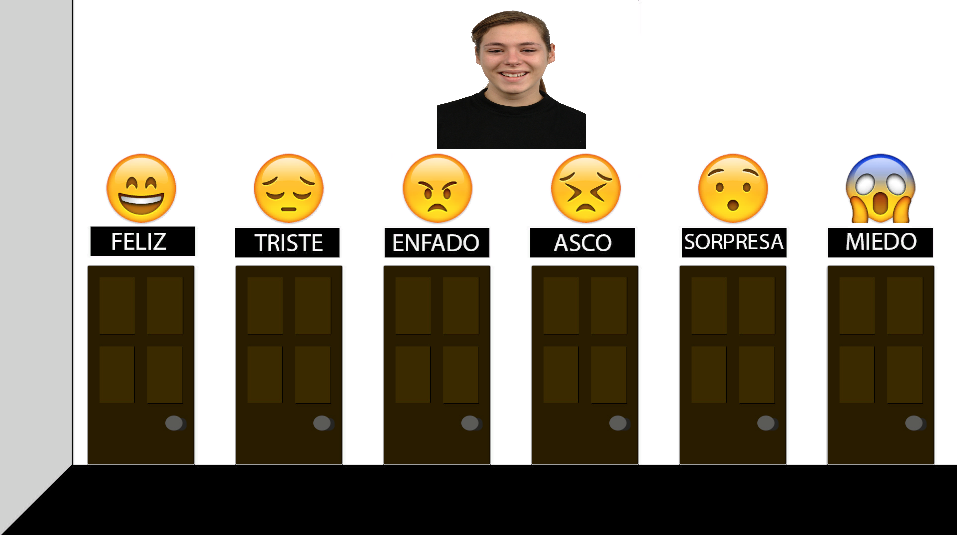
\includegraphics[width=0.85\linewidth]{Fig1.png}
\caption{Muestra de la interfaz de usuario de IDADIE en una tarea de emparejamiento emoción-cara.}
\label{fig1}
\source{Elaboración propia.}
\end{figure}

El subbloque 1.2, que incluye tareas de emparejamiento emoción-situación, está compuesto por las partes 7, 8, 9, 10, 11 y 12, e integra imágenes de componente emocional extraídas, en este caso, del banco de imágenes y sonidos del Instituto Nacional de Tecnologías Educativas y de Formación del Profesorado (INTEF) (\url{https://procomun.intef.es/bm/buscador/image/todos}). Los participantes deben relacionar una situación con la emoción que esta les sugiere.

\item \textit{Identificación de la emoción predominante en un relato}: En este bloque, los estímulos son audiovisuales. Se trata de 6 historias que el docente puede reproducir mediante el uso nativo de un motor de búsqueda en IDADIE. Tras la reproducción del relato, aparecen las 6 puertas asociadas a emociones, y, en la parte central, la imagen del cuento con el que cada participante debe emparejarlas (\Cref{fig2}). En este caso, se le pide al alumno que señale la emoción principal que le transmite la historia.

\begin{figure}[h!]
    \centering
    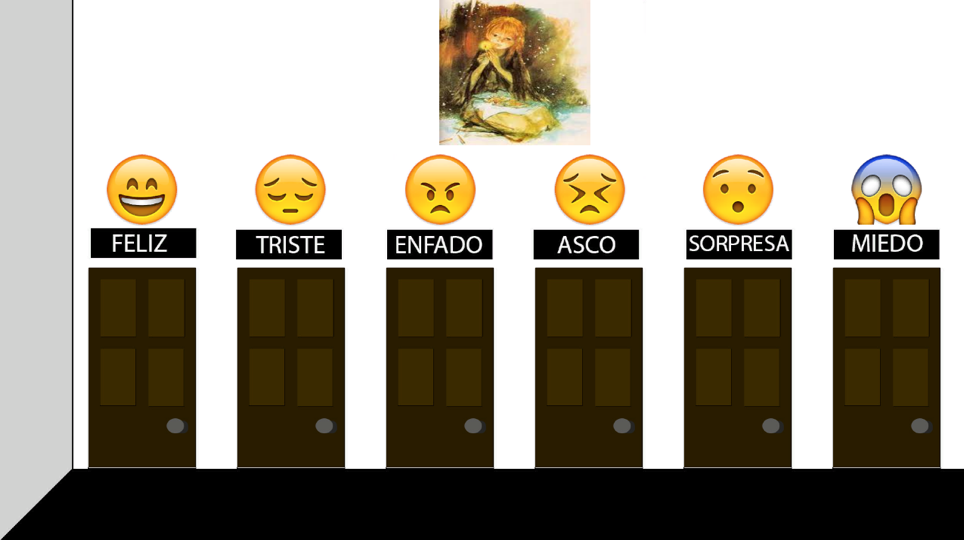
\includegraphics[width=0.85\linewidth]{Fig2.png}
    \caption{Muestra de la interfaz de usuario de IDADIE en una tarea de identificación de la emoción predominante en un relato.}
    \label{fig2}
    \source{Elaboración propia.}
\end{figure}
\end{enumerate}

Al finalizar las tareas de ambos bloques, los participantes reciben feedback a partir de su elección para que puedan autoevaluar su desempeño. No se indica “bien” / “mal”, sino que se incluye la palabra correspondiente a la emoción que deben haber identificado junto al emoticono que la representa, de manera que los participantes pueden saber por sí solos si el emparejamiento ha sido el esperado.

\subsection{Procedimiento}\label{sec-formato}
La investigación constó de tres fases diferenciadas: 
\begin{description}
\item[Fase 1. Diseño del programa computarizado] El instrumento empleado en la investigación, el videojuego IDADIE, se basó en el programa EDEMCO e implicó la adaptación al alumnado de Educación Infantil. Para ello, se utilizó un entorno simple y plano, similar al de los populares juegos de los dispositivos móviles, que, además, es apto para la mayor parte de los dispositivos táctiles y no táctiles, y puede ejecutarse en Android, Windows o Linux. 
\item[Fase 2. Pilotaje de IDADIE en un aula de infantil de 3 años] La implementación del programa en el aula para el grupo experimental se realizó en el transcurso de 2 meses y se dividió en 38 sesiones. Los materiales utilizados con el grupo control para el desarrollo de las tareas de emparejamiento de emoción-cara, emoción-objeto y emoción-situación fueron impresos y plastificados. En el caso de las tareas de identificación de emoción predominante en relatos, fue el docente-colaborador quien se encargó de reproducir y proyectar el correspondiente archivo audiovisual en clase y, posteriormente, de preguntar oralmente a los alumnos y anotar los resultados obtenidos en la evaluación que se efectuó antes y después de la intervención. 

En la intervención llevada a cabo con ambos grupos, se empleó un diario de observación en el que se fueron recogiendo las preguntas planteadas por los participantes, sus reacciones, comentarios, etc. Asimismo, tras la evaluación final, se completaron estas anotaciones con el feedback proporcionado por el grupo experimental tras haber usado IDADIE.

\item[Fase 3. Análisis de la experiencia didáctica] Al final del proceso, transcurridas 8 semanas, se realizó una evaluación final tanto en el grupo experimental como en el control para valorar la operatividad de la herramienta IDADIE. Los datos correspondientes al segundo grupo fueron solicitados al docente-colaborador, encargado de realizar las mismas tareas con el grupo control y de registrar el número de aciertos y errores. Al analizar la experiencia, se tuvieron en cuenta las opiniones del alumnado al finalizar el proceso de intervención con IDADIE.
\end{description}





\subsection{Análisis estadístico}\label{sec-modelo}
Complementariamente, se recurrió al análisis estadístico con el \textit{software} R versión 3.1.3 %(Bell Laboratories, New Jersey, NJ, USA) 
\cite{rsoftware} con objeto de determinar la significación estadística de las proporciones de aciertos que se produjeron intra- e intergrupalmente en las tareas de emparejamiento emoción-cara y emoción-objeto. Para ello, se efectuó un análisis inferencial-binominal; en concreto, se aplicó una prueba z de dos muestras para el contraste de proporciones. El nivel de significación se estableció en $p < ,05$.

\section{Resultados}\label{sec-organizacao}
Antes de emplear IDADIE en el aula con el grupo experimental, se realizó una evaluación inicial en ambos grupos. Si bien tanto en el grupo experimental como en el grupo control se completaron todas las tareas, en este apartado, se comparan intra- e intergrupalmente los resultados obtenidos únicamente en las tareas de emparejamiento emocional con caras y objetos. Así pues, se presentan los datos recogidos antes (evaluación inicial) y después (evaluación final) de la intervención con y sin IDADIE referidos a ambos conjuntos de tareas, que son las que forman el bloque 1.1 del videojuego utilizado.

Los porcentajes de acierto y error correspondientes a la evaluación inicial del grupo control quedan recogidos en la \Cref{tab01} y los del grupo experimental en la \Cref{tab02}. Como puede comprobarse, las puntuaciones en ambos grupos son similares en la evaluación inicial, lo que garantiza la homogeneidad entre grupos.

\begin{table}[h!]
\centering
\begin{threeparttable}
\caption{Evaluación inicial del grupo control.}
\label{tab01}
\begin{tabular}{l l l l l l l}
\toprule
 Caras & Felicidad & Tristeza & Enfado & Asco & Sorpresa & Miedo \\
 \midrule
\% Aciertos & 80 & 62,5 & 68,75 & 43,75 & 12,5 & 37,5 \\
\% Errores & 20 & 37,5 & 31,25 & 56,25 & 87,5 & 62,5 \\
Objetos & & & & & & \\
\% Aciertos & 68,75 & 56,25 & 50 & 56,25 & 25 & 50 \\
\% Errores & 31,25 & 43,75 & 50 & 43,75 & 75 & 50 \\
\bottomrule
\end{tabular}
\source{Elaboración propia.}
\end{threeparttable}
\end{table}

\begin{table}[h!]
\centering
\begin{threeparttable}
\caption{Evaluación inicial del grupo experimental.}
\label{tab02}
\begin{tabular}{l l l l l l l}
\toprule
 Caras & Felicidad & Tristeza & Enfado & Asco & Sorpresa & Miedo \\
 \midrule
\% Aciertos & 81,25 & 68,75 & 43,75 & 31,25 & 50 & 31,25  \\
\% Errores & 18,75 & 31,25 & 56,25 & 68,75 & 50 & 68,75  \\
Objetos & & & & & & \\
\% Aciertos & 68,75 & 62,5 & 31,25 & 56,25 & 43,75 & 62,5 \\
\% Errores & 31,25 & 37,5 & 68,75 & 43,75 & 56,25 & 37,5 \\
\bottomrule
\end{tabular}
\source{Elaboración propia.}
\end{threeparttable}
\end{table}

Los resultados relativos a la evaluación final del grupo control se recogen en la \Cref{tab03} y los que obtuvo el grupo experimental en la \Cref{tab04}.

\begin{table}[h!]
\centering
\begin{threeparttable}
\caption{Evaluación final del grupo control.}
\label{tab03}
\begin{tabular}{l l l l l l l}
\toprule
 Caras & Felicidad & Tristeza & Enfado & Asco & Sorpresa & Miedo \\
 \midrule
\% Aciertos & 69,23 & 50 & 64,28 & 14,28 & 35,71 & 21,42 \\
\% Errores & 30,76 & 50 & 35,71 & 85,71 & 64,28 & 78,57 \\
Objetos & & & & & & \\
\% Aciertos & 57,14 & 50 & 35,71 & 50 & 0 & 14,28 \\
\% Errores & 42,85 & 50 & 64,28 & 50 & 100 & 85,71 \\
\bottomrule
\end{tabular}
\source{Elaboración propia.}
\end{threeparttable}
\end{table}

\begin{table}[h!]
\centering
\begin{threeparttable}
\caption{Evaluación final del grupo experimental.}
\label{tab04}
\begin{tabular}{l l l l l l l}
\toprule
 Caras & Felicidad & Tristeza & Enfado & Asco & Sorpresa & Miedo \\
 \midrule
\% Aciertos & 100 & 66,67 & 80 & 80 & 86,67 & 73,33 \\
\% Errores & 0 & 33,3 & 20 & 20 & 13,33 & 26,67 \\
Objetos & & & & & & \\
\% Aciertos & 73,33 & 100 & 93,33 & 93,33 & 66,67 & 86,67 \\
\% Errores & 26,67 & 0 & 6,67 & 6,67 & 33,33 & 13,33 \\
\bottomrule
\end{tabular}
\source{Elaboración propia.}
\end{threeparttable}
\end{table}

De acuerdo con las diferencias entre la evaluación inicial y final en el grupo control (\Cref{tab01,tab03}), en las tareas de emparejamiento emoción-cara resultó significativo ($p < ,05$) el reconocimiento de la sorpresa ($z = 3,15$) por el mayor número de aciertos producido. Sin embargo, fue estadísticamente significativo, pero por el mayor de número de errores cometido al emparejar emoción-cara antes y después de la intervención, el peor reconocimiento del asco ($z = 3,9$). En las tareas de emparejamiento emoción-objeto, este retroceso del grupo control se asoció a las emociones de enfado ($z = -1,67$), miedo ($z = -4,54$) y sorpresa ($z = -4,6$); en este caso, el peor reconocimiento del asco no fue estadísticamente significativo. 

En relación con el desempeño del grupo experimental, en las tareas de emparejamiento emoción-cara, al comparar los resultados iniciales y finales (\Cref{tab02,tab04}), se evidencian avances significativos ($p < ,05$) al reconocer las siguientes emociones: enfado ($z = -5,59$), asco ($z = -2,93$), sorpresa ($z = -3,28$) y miedo ($z = -4,1$). La felicidad fue adecuadamente reconocida antes de la intervención (81,25~\%), pero alcanzó un 100~\% de aciertos en la evaluación final. Solo disminuyó el número de aciertos en la tarea de emparejamiento tristeza-cara, si bien este retroceso fue muy leve y no es estadísticamente significativo. En las tareas de emparejamiento emoción-objeto, fue significativo el aumento de aciertos asociado a la identificación de las siguientes emociones: tristeza ($z = -2,89$), enfado ($z = -5,6$), asco ($z = -2,93$), sorpresa ($z = -2,1$) y miedo ($z = -1,95$). Como en las tareas de emparejamiento emoción-cara, la felicidad fue reconocida por más de la mitad de los participantes antes de usar IDADIE; pero también mostró un progreso en la evaluación final, aunque no resulta estadísticamente significativo.

Si se atiende a las puntuaciones de acuerdo con la sumatorio del total de puntuaciones porcentuales obtenidas en cada emoción, como refleja la \Cref{fig3}, al realizar el contraste intragrupal, el grupo control ha mostrado un retroceso en el número de aciertos producidos en las tareas de emparejamiento emoción-cara ($z = 1,89$; $p < ,05$) y emoción-objeto ($z = 4,54$; $p < ,05$), si bien en las tareas de emparejamiento emoción-objeto este retroceso ha sido más acusado que en las tareas de emparejamiento emoción-cara.

\begin{figure}[h!]
    \centering
    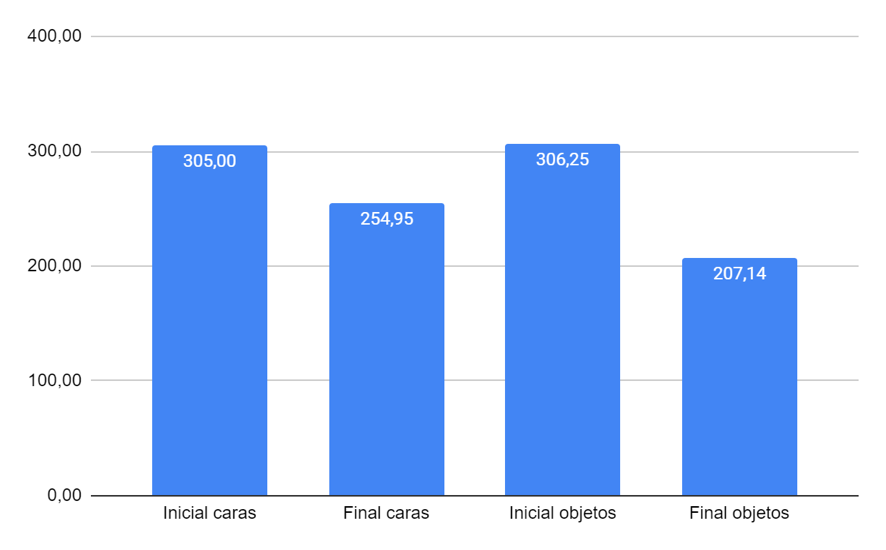
\includegraphics[width=0.85\linewidth]{Fig3.png}
    \caption{Sumatorio total porcentual del grupo control.}
    \label{fig3}
    \source{Elaboración propia.}
\end{figure}

La \Cref{fig4} permite comprobar cómo el grupo experimental ha mejorado en la ejecución de las tareas de emparejamiento de emoción-cara ($z = -6,18$; $p < ,05$) y emoción-objeto ($z = -6,46$; $p < ,05$), pues, al comparar los datos de la evaluación inicial con los de la final, el contraste es estadísticamente significativo; en este caso, el avance ha sido algo más acusado al reconocer emociones vinculadas a objetos.

\begin{figure}[h!]
    \centering
    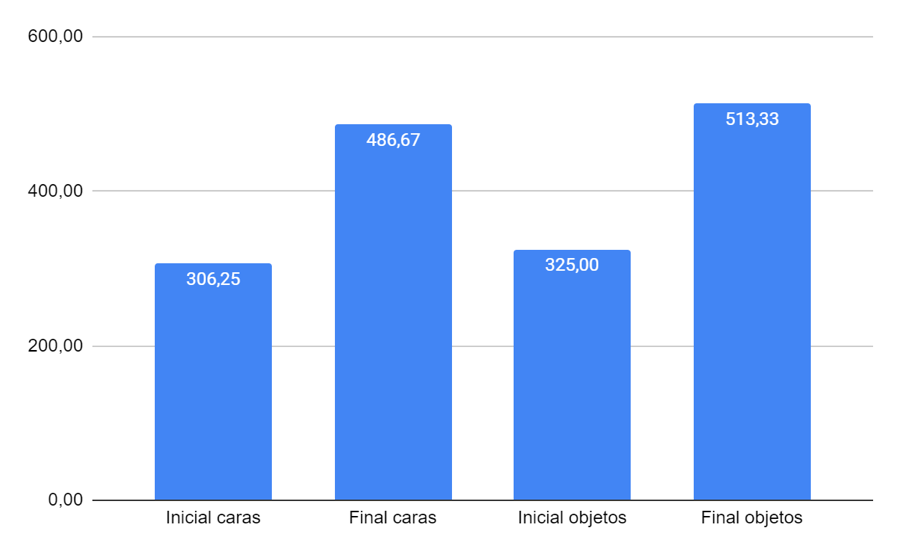
\includegraphics[width=0.85\linewidth]{Fig4.png}
    \caption{Sumatorio total porcentual del grupo experimental.}
    \label{fig4}
    \source{Elaboración propia.}
\end{figure}

Por último, en el grupo control, las puntuaciones en las tareas de emparejamiento emoción-cara en la evaluación inicial fueron de 305 puntos, frente a los 306,25 del grupo experimental. En las tareas de emparejamiento emoción-objeto, el grupo control puntuó 306,25, y el grupo experimental, 325. Por su parte, las puntuaciones finales totales en las tareas de emparejamiento emoción-cara fueron de 254,95 puntos en el grupo control y de 486,67 en el grupo experimental. En estas tareas, el grupo para cuya intervención se ha empleado IDADIE ha aumentado su capacidad de identificar emociones en 231,72 puntos ($z = -8,74$; $p < ,05$). En las tareas de emparejamiento emoción-objeto, el grupo control obtuvo 207,14 puntos, frente a los 513,33 del grupo experimental; la diferencia total fue de 306,19 puntos ($z = -11,24$; $p < ,05$). Atendiendo a la comparación intergrupal de la evaluación inicial y final, los avances en el reconocimiento emocional experimentados por el grupo que se ha beneficiado del uso de IDADIE han sido significativos, más aún en el caso de las tareas de emparejamiento emoción-objeto.

\section{Discusión y conclusiones}\label{sec-titulo}
Esta intervención ha buscado comprobar si existen mejoras en la ejecución de tareas de componente emocional a partir de la implementación de un programa diseñado con ese propósito, IDADIE, en un aula de Educación Infantil. En concreto, se han comparado intra- e intergrupalmente los resultados obtenidos en dos conjuntos de tareas de emparejamiento: a. emoción-cara y b. emoción-objeto. 

Teniendo en cuenta que la evaluación inicial reveló que existía homogeneidad en los resultados del grupo control y experimental, y que en la evaluación final encontramos diferencias consistentes, se cumple la hipótesis 1 debido a que el grupo experimental, en el que se usó IDADIE, mostró mayores avances que el grupo control en el reconocimiento de emociones vinculadas tanto a caras como a objetos. Asimismo, se valida la hipótesis 2, ya que el grupo experimental evoluciona significativamente al comparar la evaluación inicial y la final; sobre todo, este progreso fue más destacado al lograr emparejar emociones con objetos. 

En el caso del grupo control, solo la identificación de una de las 6 emociones, la sorpresa, mejoró de manera sustancial al comparar la evaluación inicial con la final al realizar el emparejamiento emoción-cara, y se cometió un mayor número de errores al identificar el asco. Además, en las tareas de emparejamiento emoción-objeto, también fue significativo el menor número de aciertos vinculado a la identificación del enfado, el miedo y la sorpresa. Al buscar las causas de este retroceso, el docente-colaborador, que se encargó de intervenir en el grupo control con material impreso, manifestó que los emoticonos que utilizó asociados a las emociones que los participantes debían identificar variaron para algunas de ellas entre la evaluación inicial y final.

Al cotejar el desempeño del grupo experimental entre la evaluación inicial y final, el alumnado participante planteó dudas relacionadas con la emoción tristeza al ejecutar la tarea de emparejamiento emoción-cara; concretamente, en el aula se observó que los alumnos confundían la emoción tristeza con enfado. De hecho, este grupo mostró mejoras al reconocer todas las emociones en las tareas de emparejamiento emoción-cara y emoción-objeto, excepto en este caso. Aunque la diferencia no es estadísticamente significativa (-2,08 puntos porcentuales), debe plantearse la revisión del contenido visual asociado a esta emoción en IDADIE. 

Donde más progresó el grupo experimental al identificar emociones faciales fue en el caso del asco y el miedo, seguidos de la sorpresa y el enfado, mientras que los resultados obtenidos en felicidad y tristeza no mostraron una mejora estadísticamente significativa. Un dato curioso asociado a la tarea de emparejamiento emoción-objeto es que el grupo control tuvo un 0~\% de aciertos al reconocer la sorpresa, frente al 66,67~\% de aciertos del grupo experimental. Esto puede deberse a que, según señalan los teóricos de las emociones \cite{goleman_inteligencia_2021,izard_il_1977}, la identificación de la sorpresa resulta más problemática.

Atendiendo a cómo se desarrollaron las sesiones y al \textit{feedback} de los alumnos del grupo experimental al finalizar la experiencia didáctica, es posible sostener que el uso de IDADIE en el aula ha fomentado la participación, les ha resultado atractivo y ha supuesto una disminución de la fatiga. En este sentido, percibimos que los niños logran prestar más atención durante más tiempo en clase cuando usamos esta herramienta que ante una actividad convencional, algo que corroboró el docente-colaborador al comparar su intervención sin IDADIE con la nuestra. También nos percatamos de que los niños están más motivados durante la realización de la actividad, lo que podría verse reflejado en un aumento del rendimiento en el aprendizaje y en un mejor manejo de las emociones \cite{norman_emotion_2002,pagulayan_user-centered_2003}.

En definitiva, optimizando el instrumento diseñado para la investigación y probando la herramienta IDADIE en una muestra más amplia, su incorporación futura en aulas de Educación Infantil puede resultar muy ventajosa en materia de desarrollo emocional y gozar de aceptación por parte tanto del alumnado como del profesorado, así como repercutir en la motivación por aprender que manifiestan al usar el instrumento.



\printbibliography\label{sec-bib}
%conceptualization,datacuration,formalanalysis,funding,investigation,methodology,projadm,resources,software,supervision,validation,visualization,writing,review
\begin{contributors}[sec-contributors]
\authorcontribution{Gabriel Artés Ordoño}[investigation,projadm,formalanalysis,software,writing]
\authorcontribution{Francisco J. Rodríguez Muñoz}[investigation,projadm,formalanalysis,methodology,supervision,review]
\authorcontribution{Gemma Quirantes Gutiérrez}[investigation,formalanalysis,resources,writing]
\end{contributors}
\end{document}
